\chapter{Anexos}	
		\section{Capturas de Pantalla de las contribuciones al código}
			A continuación se muestra las capturas de pantalla de algunas de las
			contribuciones al código fuente en el repositorio en la nube (Bitbucket):
			
			\begin{figure}[H]
			    \centering
				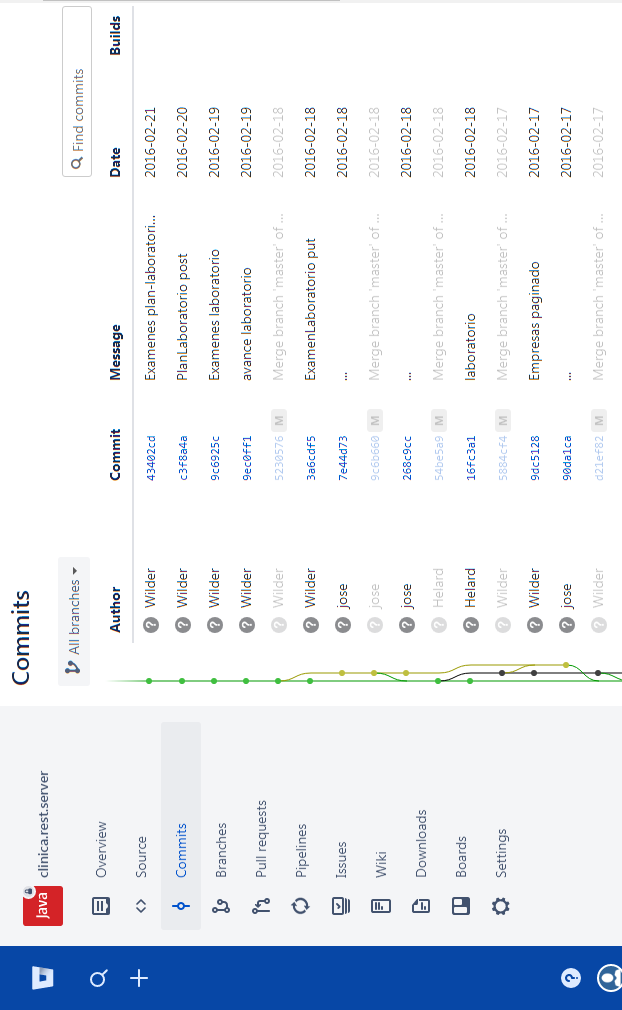
\includegraphics[width=13cm]{../imgs/ui/bitbucket-back.png}
				\caption{Pantalla contribución backend}
				\label{figure:bitbucket-back}
			\end{figure}
			
			\begin{figure}[H]
			    \centering
				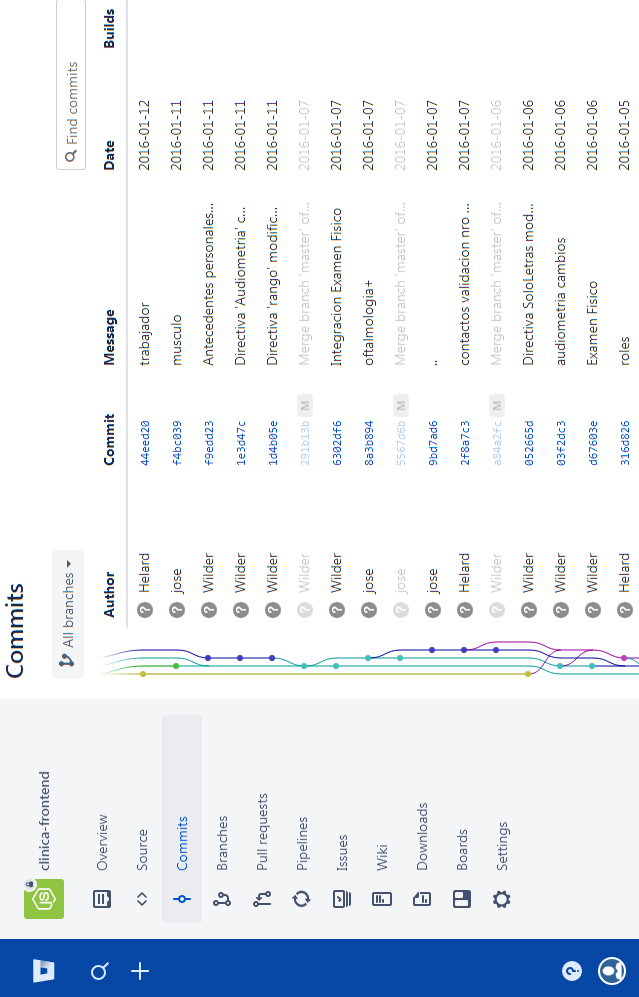
\includegraphics[width=13cm]{../imgs/ui/bitbucket-front.png}
				\caption{Pantalla contribución frontend}
				\label{figure:bitbucket-front}
			\end{figure}
		
		\section{Capturas de Pantalla del Sistema}
			A continuación se muestra algunas de las capturas de pantalla del sistema:
			
			\begin{figure}[H]
			    \centering
				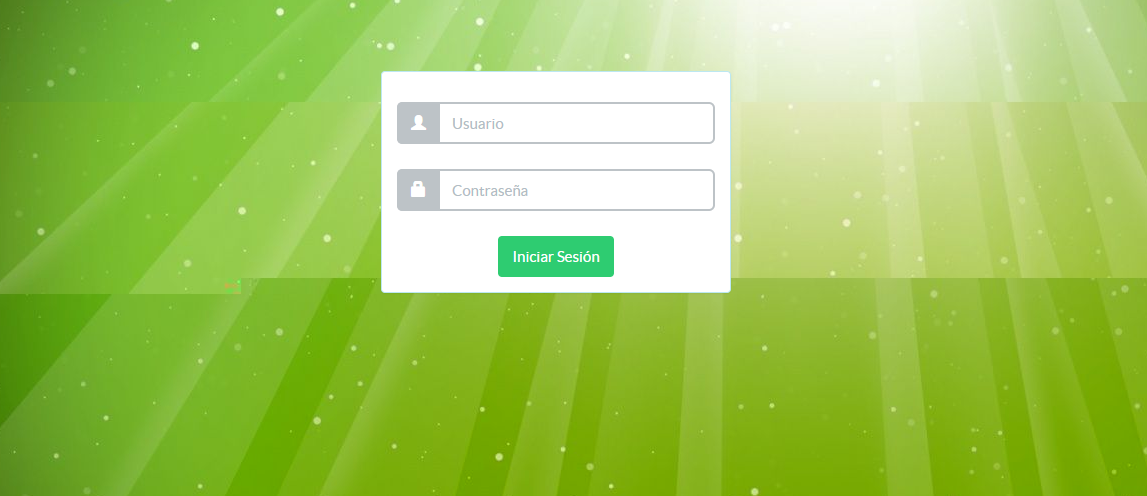
\includegraphics[width=18cm]{../imgs/ui/login.png}
				\caption{Pantalla login}
				\label{figure:login}
			\end{figure}
			
			\begin{figure}[H]
			    \centering
				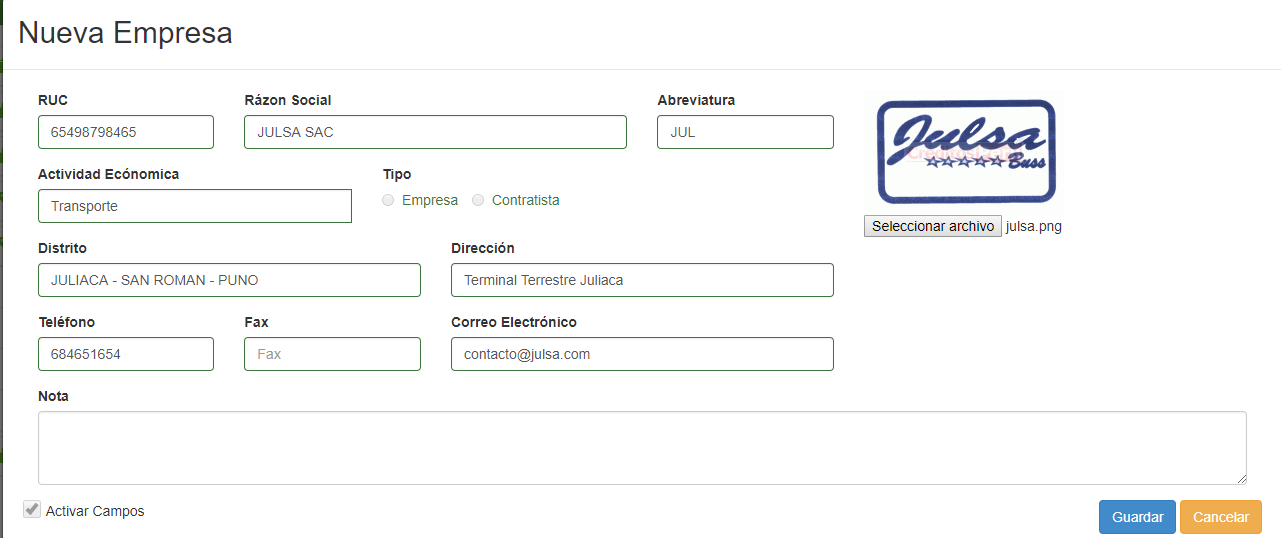
\includegraphics[width=18cm]{../imgs/ui/nueva-empresa.png}
				\caption{Pantalla nueva empresa}
				\label{figure:nueva-empresa}
			\end{figure}
			
			\begin{figure}[H]
			    \centering
				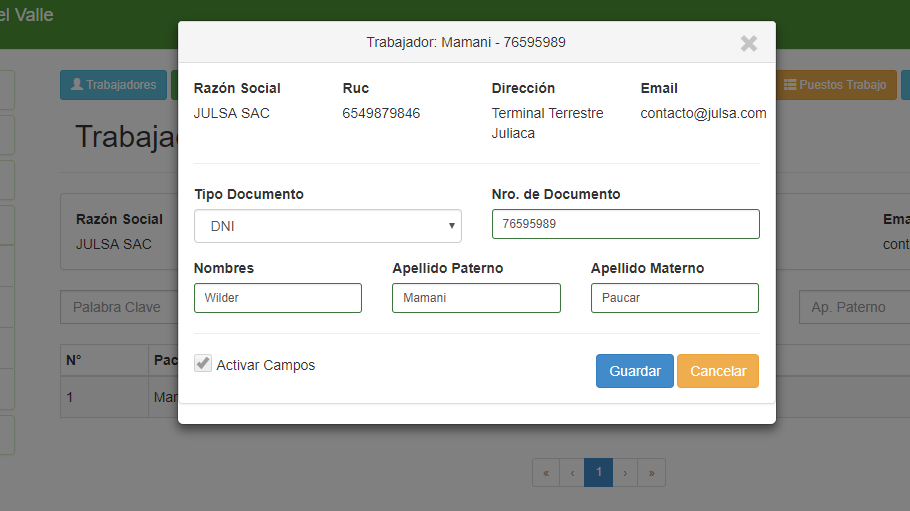
\includegraphics[width=18cm]{../imgs/ui/paciente.png}
				\caption{Pantalla nuevo paciente}
				\label{figure:paciente}
			\end{figure}
			
			\begin{figure}[H]
			    \centering
				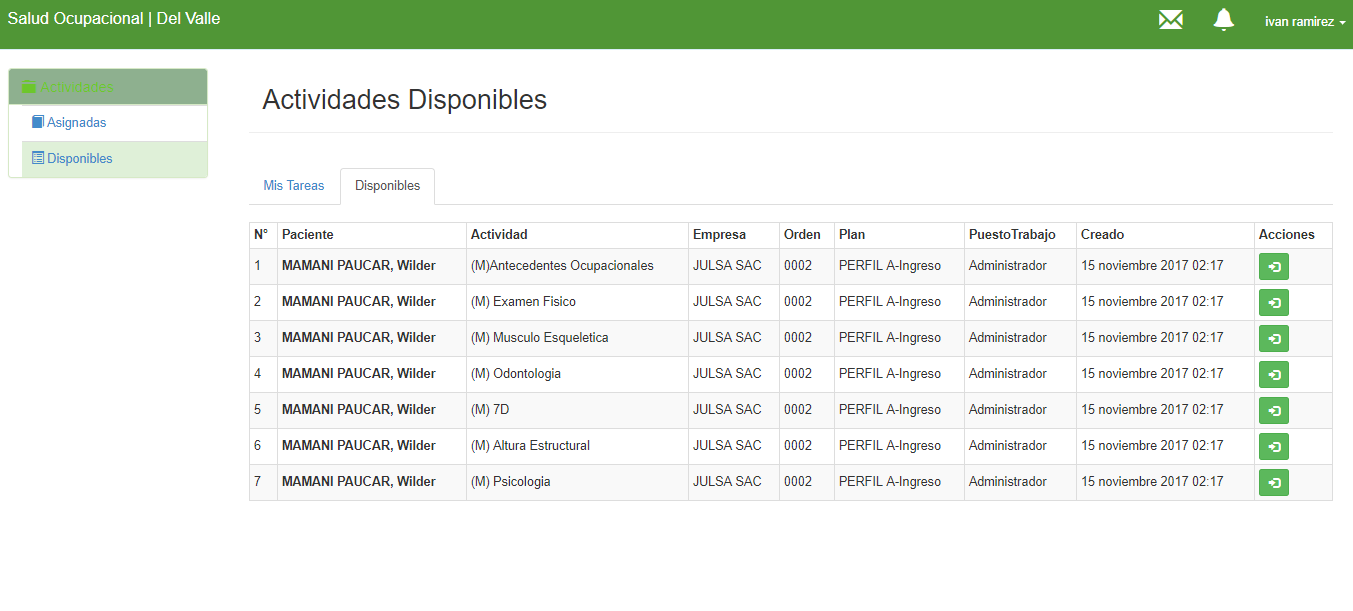
\includegraphics[width=18cm]{../imgs/ui/disponibles.png}
				\caption{Pantalla exámenes a realizar}
				\label{figure:disponibles}
			\end{figure}
			
			\begin{figure}[H]
			    \centering
				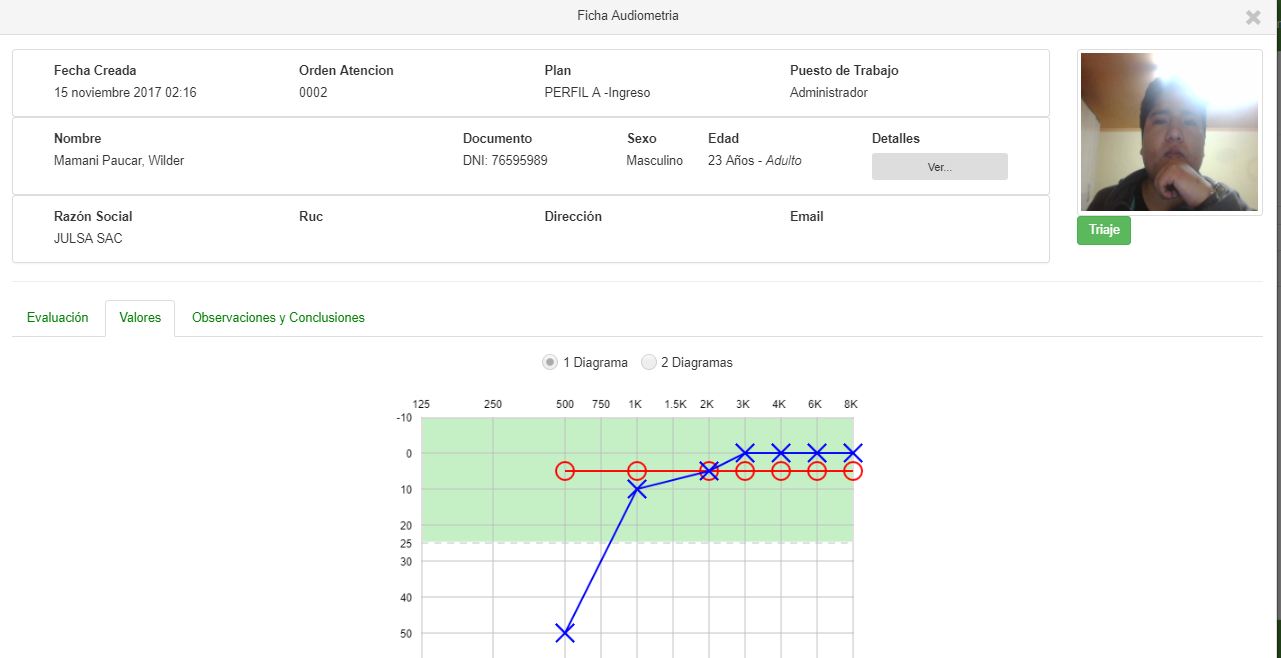
\includegraphics[width=18cm]{../imgs/ui/audiometria.png}
				\caption{Pantalla examen audiometría}
				\label{figure:audiometria}
			\end{figure}
			
			\begin{figure}[H]
			    \centering
				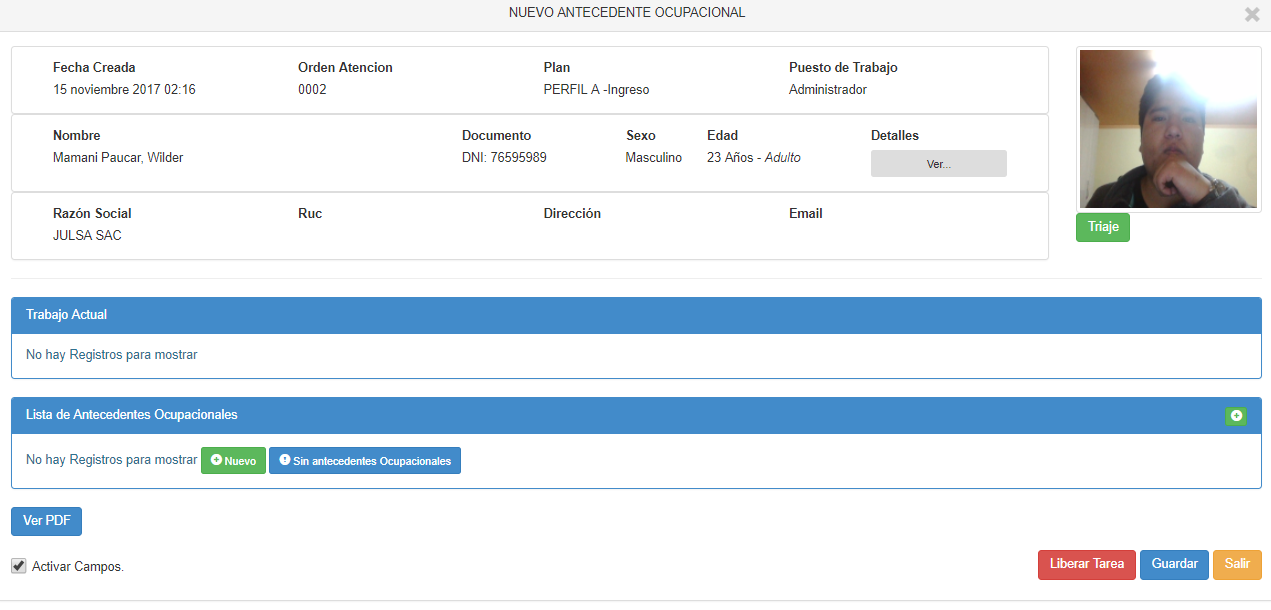
\includegraphics[width=18cm]{../imgs/ui/ocupacional.png}
				\caption{Pantalla antecedentes ocupacionales}
				\label{figure:ocupacional}
			\end{figure}
			
			
			
		\section{Capturas de Pantalla del Código}
			A continuación se muestra algunas de las capturas de pantalla del código
			fuente (frontend y backend:
			
			\begin{figure}[H]
			    \centering
				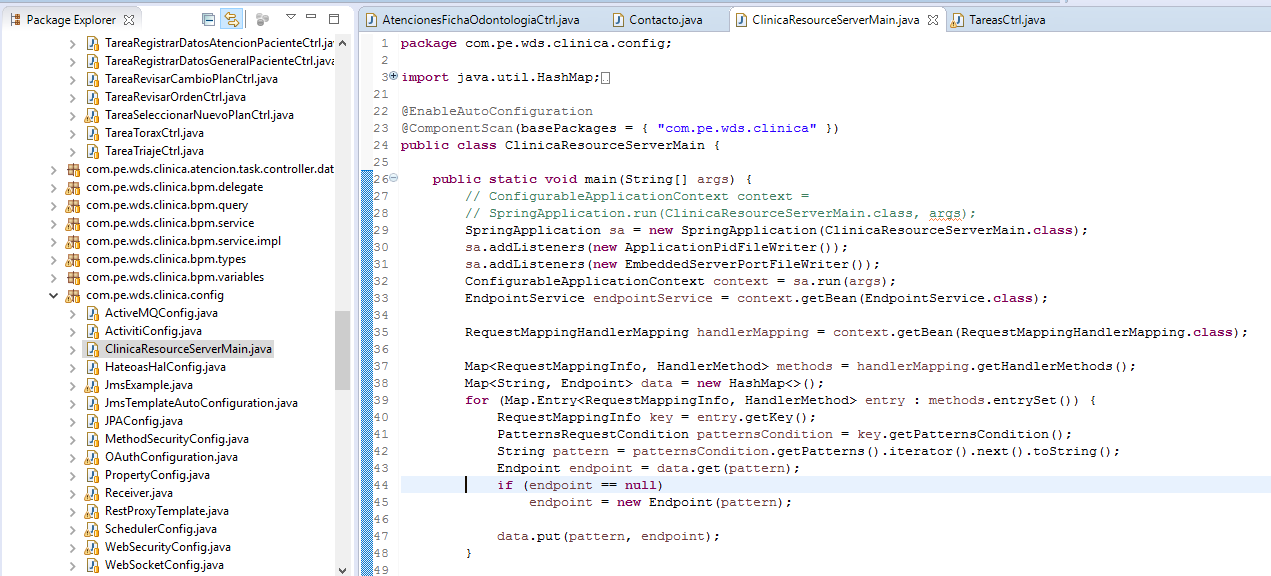
\includegraphics[width=18cm]{../imgs/codigo/back-main.png}
				\caption{Pantalla backend código principal}
				\label{figure:back-main}
			\end{figure}
			
			\begin{figure}[H]
			    \centering
				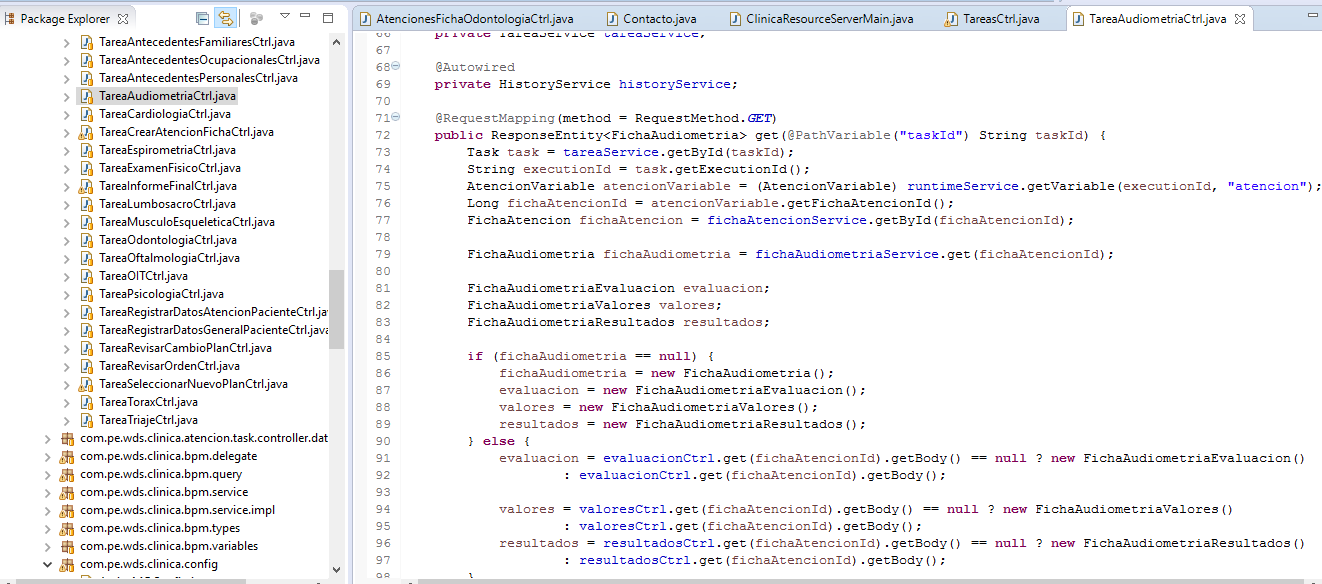
\includegraphics[width=18cm]{../imgs/codigo/back-ctrl.png}
				\caption{Pantalla backend código controlador audiometría}
				\label{figure:back-ctrl}
			\end{figure}
			
			
			\begin{figure}[H]
			    \centering
				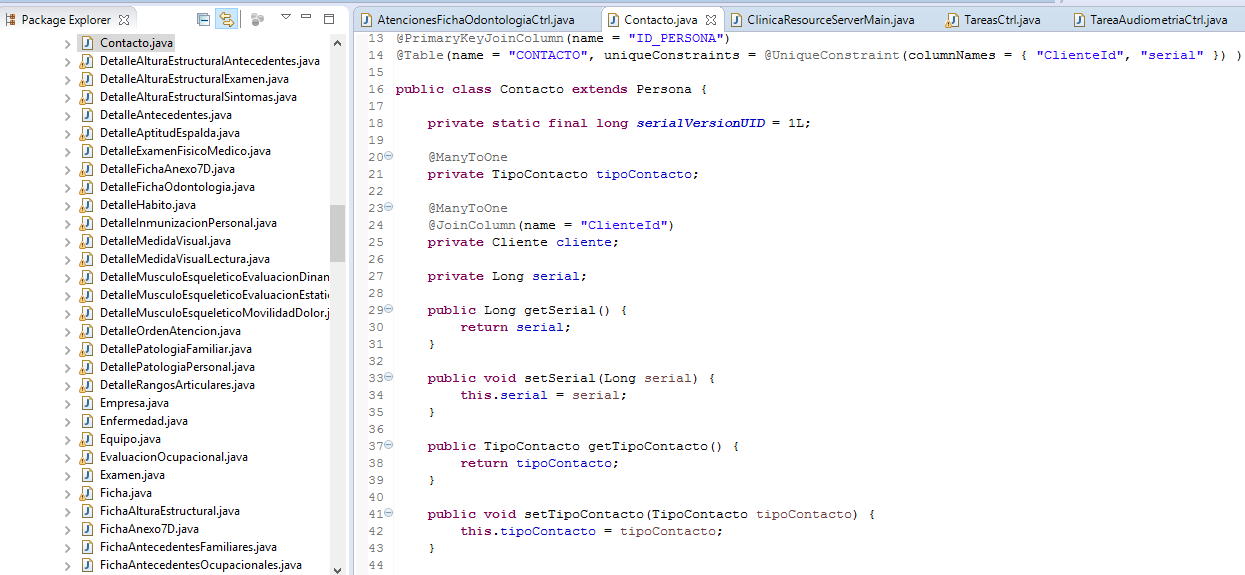
\includegraphics[width=18cm]{../imgs/codigo/back-entity.png}
				\caption{Pantalla backend código entidad contacto}
				\label{figure:back-entity}
			\end{figure}
			
			\begin{figure}[H]
			    \centering
				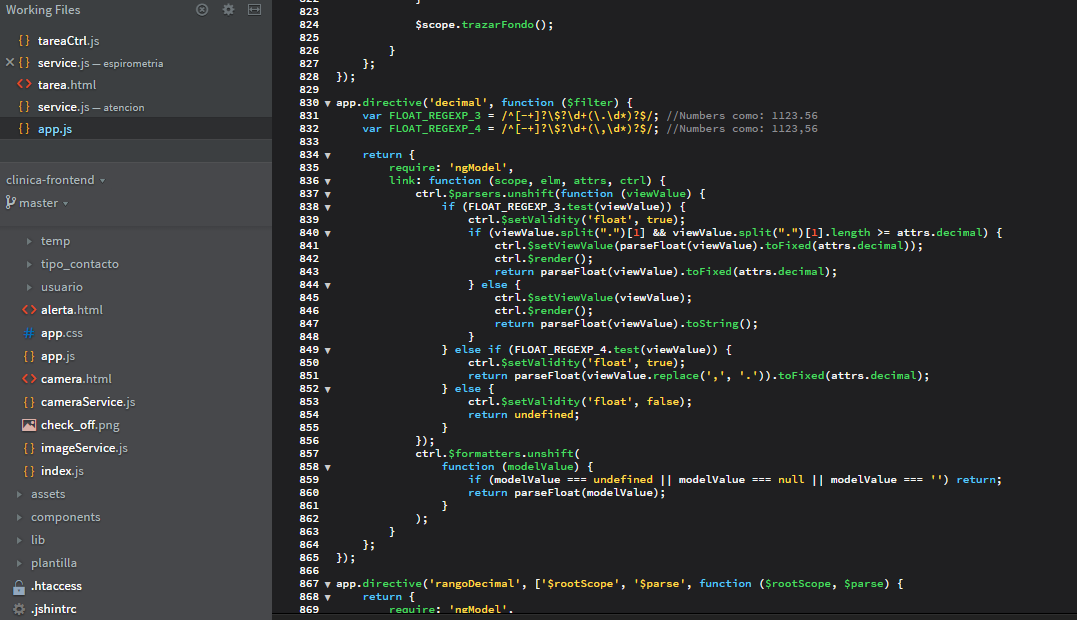
\includegraphics[width=18cm]{../imgs/codigo/front-main.png}
				\caption{Pantalla frontend código principal}
				\label{figure:front-main}
			\end{figure}
			
			\begin{figure}[H]
			    \centering
				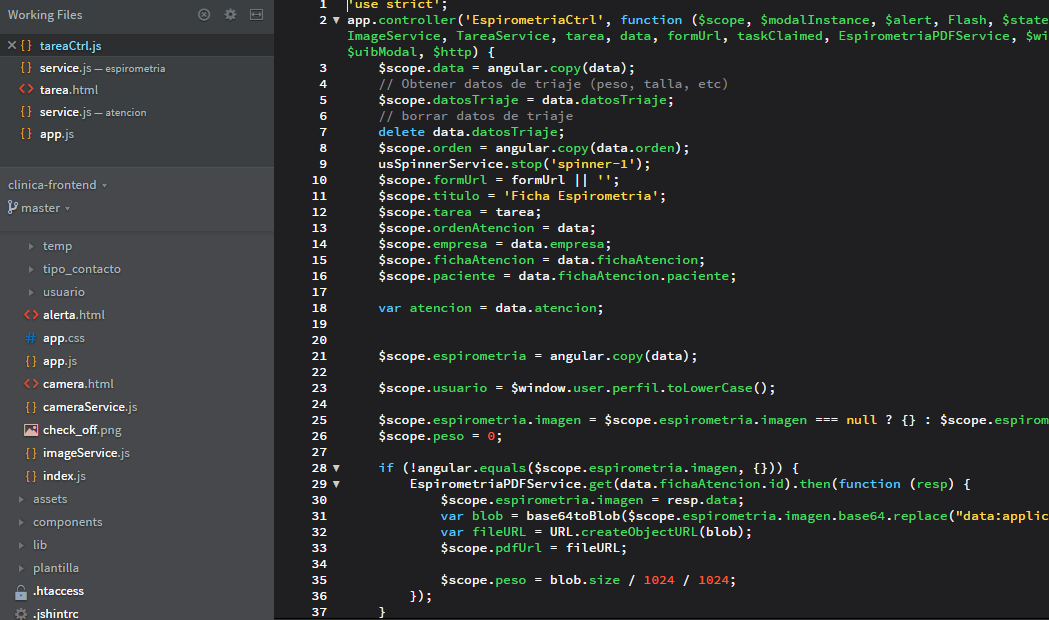
\includegraphics[width=16cm]{../imgs/codigo/front-ctrl.png}
				\caption{Pantalla frontend código controlador espirometría}
				\label{figure:front-ctrl}
			\end{figure}
			
			\begin{figure}[H]
			    \centering
				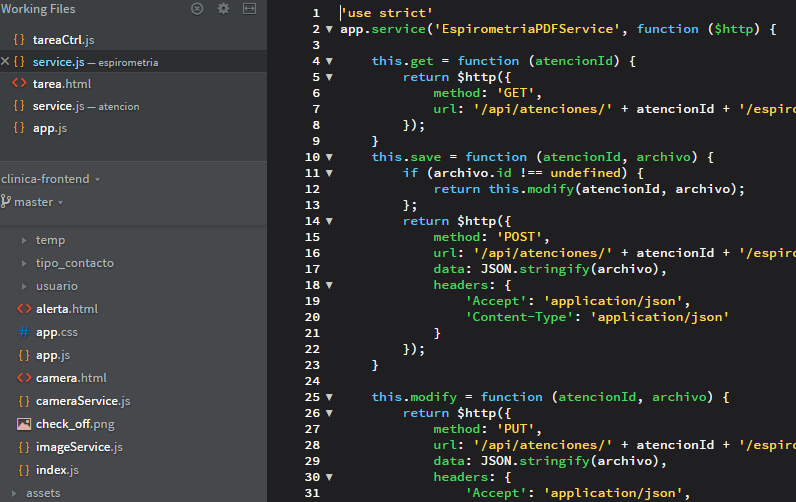
\includegraphics[width=15cm]{../imgs/codigo/front-service.png}
				\caption{Pantalla frontend código comunicación con el backend}
				\label{figure:front-service}
			\end{figure}